\documentclass[margin,line]{res}
\usepackage{graphicx,array}
\usepackage{hyperref}

\oddsidemargin -.5in
\evensidemargin -.5in
\textwidth=6.0in
\itemsep=0in
\parsep=0in
\topmargin=0in
\topskip=0in


\hypersetup{pdfborderstyle={/S/U/W 1}}



\begin{document}

	\name{\Huge{K V Sai \textbf{Akhil}}} \hfill 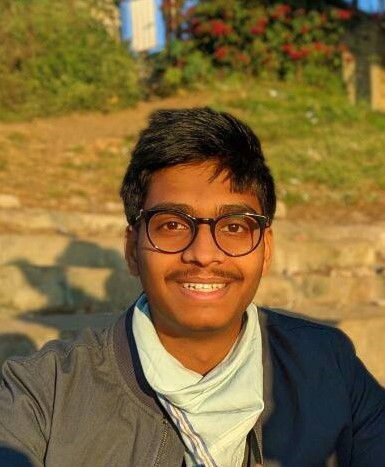
\includegraphics[scale=0.35]{photo.jpg}
	\vspace{-.25in}


	\begin{resume}


		\section{\sc contact information}
			\begin{tabular}{@{}p{3.5in}p{3.5in}}
				\#3117, NH-3,          & Phone:  +91 9620943665 \\
				BMSET Hostel,        & E-mail: \href{saiakhilkv999@gmail.com}{saiakhilkv999@gmail.com} \\
				opp. Allahabad Bank, & Github: \href{https://github.com/kvsaiakhil}{kvsaiakhil}\\
				Basavanagudi, & \\
				Bangalore - 560019 \\
				Karnataka\\
			\end{tabular}

		\section{\sc objective}
			\textbf{Looking for an internship to enhance my technical skills and gain real world problem solving experience in the field of computer vision and embedded systems.}

		\section{\sc  education}
			\begin{itemize}
				\item \textbf{Undergraduate (B.E) --- Electronics and Communication Engineering} \newline
					\small B. M. S College of Engineering, Bengaluru $\vert$ Visvesvaraya Technological University $\vert$ 2020 (expected) \newline
					\null\hfill \textbf{5\textsuperscript{th} Sem. CGPA 8.9}

				\item \textbf{Pre University --- PCMC (Computer Science)} \newline
					\small AECS Magnolia Maaruti PU College, Bengaluru $\vert$ Karnataka Pre University Board $\vert$ 2016 \newline
					\null\hfill \textbf{Aggregate 90.33\%}

				\item \textbf{10\textsuperscript{th}} \newline
					\small Dream World School, Ballari, Karnataka $\vert$ CBSE $\vert$ 2014 \newline
					\null\hfill \textbf{GPA 9.8}
			\end{itemize}

		\section{\sc projects}
			
			\begin{enumerate}

				\item \textbf{TADPOL $\vert$ Electronic prototyping platform (similar to Arduino Nano) based on Nuvoton W78E052DDG Microcontroller (8051 Architecture) } \newline \url{www.bautomateindia.com} 
					\begin{itemize}
						\item Integrated USB to TTL converter onto the breakout board  $\vert$ Schematic Design using EasyEDA 
						\item Embedded C programming
					\end{itemize}
					\null \hfill \textbf{Team of 8 $\vert$ Aug 2018 - Jan 2019} \newline
				\item \textbf{Solar Chulha Android App  $\vert$  Solar Chulha Challange, ONGC}
					\begin{itemize}	
						\item Android Application to control Solar Chulha  $\vert$  Android Studio
					\end{itemize}
					\null \hfill \textbf{Team of 2 $\vert$ Jan 2018 - March 2018} \newline
				\item \textbf{MINI PROJECTS}
					\begin{enumerate}
						\item RF Based Home Automation System $\vert$ Team of 4 $\vert$ Aug 2017 - Sept 2017
						\item Yi Camera Trigger using ESP 8266 12E via Pixhawk Flight Controller for Capturing Image from a Quadcopter. $\vert$ Team of 2 $\vert$ April 2019 - Present
					\end{enumerate}
			\end{enumerate}

		\section{\sc training}
	
			\begin{itemize}
				\item \textbf{Deep Neural Networks for Computer Vision, NASSCOM Collaborative} $\vert$ EIP 3.0 Phase 1 \newline
				\null \hfill \textbf{Feb 2019 - Present} \newline
			\end{itemize}

		\section{\sc internship}

			\begin{itemize}
				\item \textbf{Firmware Developer $\vert$ 1 month duration $\vert$ NGX Technologies Private Ltd.,}  \newline
					\begin{itemize}
						\item Application Specific firmware development for handheld billing/ticketing machine (HTM 210) $\vert$ Application: Electricity Billing
						\item Programming Language: Embedded C
					\end{itemize}
				\null \hfill \textbf{June 2018} \newline	
			\end{itemize}

		\section{\sc technical skills}

			\begin{itemize}
				\item \textbf{Programming Languages}
				\begin{itemize}
					\item Proficient: C, C++
					\item Intermediate: Python
					\item Familiar: MATLAB, Assembly (8051), Java, HTML, Verilog, \LaTeX
				\end{itemize}
				\item \textbf{Software Tools}
				\begin{itemize}
					\item Arduino IDE, LT Spice, Easy EDA, Git, ROS Kinetic, Keil $\mu$Vision, MATLAB, Xilinx Verilog, Android Studio.
				\end{itemize}
				\item \textbf{Hardware Platforms}
				\begin{itemize}
					\item TADPOL (Nuvoton 8051 W78E052DDG based), Arduino, Raspberry Pi, NODE MCU ESP8266.  
				\end{itemize}
			\end{itemize}



\end{resume}
\end{document}
